%\documentclass[a4paper,english,11pt,twoside]{article}
\documentclass[a4paper,english,11pt]{article}

\usepackage[utf8]{inputenc}
\usepackage[T1]{fontenc, url}
\usepackage[english]{babel}
%\usepackage{epsfig}
\usepackage{graphicx}
\usepackage{amsmath}
\usepackage{mathtools}
\usepackage{pstricks}
\usepackage{subfig}
\usepackage{epstopdf}
\usepackage{varioref}
\usepackage{listings}
\usepackage{xcolor}
\usepackage{float}
\usepackage[]{mcode}
\usepackage{verbatim}
\lstset{ 
  captionpos=b,
  frame=tb,
  numbers=left}
\urlstyle{sf}
\usepackage[margin=1 in]{geometry} % Setter margene til word standard

\usepackage{ifikompendiumforside}


\newcommand{\tab}[1]{\hspace{.2\textwidth}\rlap{#1}}

%%%%%%%%%%%%%%%%%% END HEADER

\title{Laboratory Assignment 2}
\subtitle{INF4411\\ 
          Analog Microelectronics}

\author{
\begin{tabular}{ r c l }
  Rikesh Chauhan & & rikesh.chauhan@fys.uio.no\\
  Espen Klein Nilsen & & e.a.k.nilsen@fys.uio.no\\
  Vegard Midtbøen & & vegard.midtboen@fys.uio.no
\end{tabular}
}
%{Rikesh Chauhan rikesh.chauhan@fys.uio.no\\
%	Espen Klein Nilsen e.a.k.nilsen@fys.uio.no\\
%	Vegard Midtbøen vegard.midtboen@fys.uio.no} 

\begin{document}
\ififorside
        
\section{Task 1}

\colorbox{red!30}{FIXME}\\
In order to get a voltage reference to V$_{p_bias1}$, we used a potentiometer as seen in figure \ref{fig:sch:task1}.
\colorbox{red!30}{ENDFIXME}\\

For the task, we used a Vdd = 5V, which is enough for this task (Vds = 5V). 
This voltage is fixed trough the whole experiment. In the task it is given that the transitor should supply a 20mA current. 
In order too get this current we created the circut shown in figure \ref{fig:sch:task1}. In this setup we tuned the potensiometer to set the bias voltage V$_{p_bias1}$.

The results for the experiment is shown in the figure REF*******************
The minimal Vout for this cuircuit to act as an current source is  **************
Since we probably want to be able to have an AC input, we need some headroom in order to acomodate the signal, both in the positive and negative direction from the setpoint.
The amount of headroom should be big enugh so the transistor never goes out of the active region.*********

\colorbox{red!30}{FIXME}\\
When we selected the V$_{p_bias1}$, we coupled up the circuit as shown in figure (figure ref). In the labdescription it was
gived that the bias current should be 20$\mu$A for the transistor to be in the active region.
V$_{p\_bias}$ = 1.196V\\
rds = 391k$\varOmega$\\
minimal V$_{out}$ = 1.818V\\
Headroom voltage is required to keep the device in active region MORE DETAILS!\\
\colorbox{red!30}{ENDFIXME}\\
    
\begin{figure}[htbp]
 \centering
  \fbox{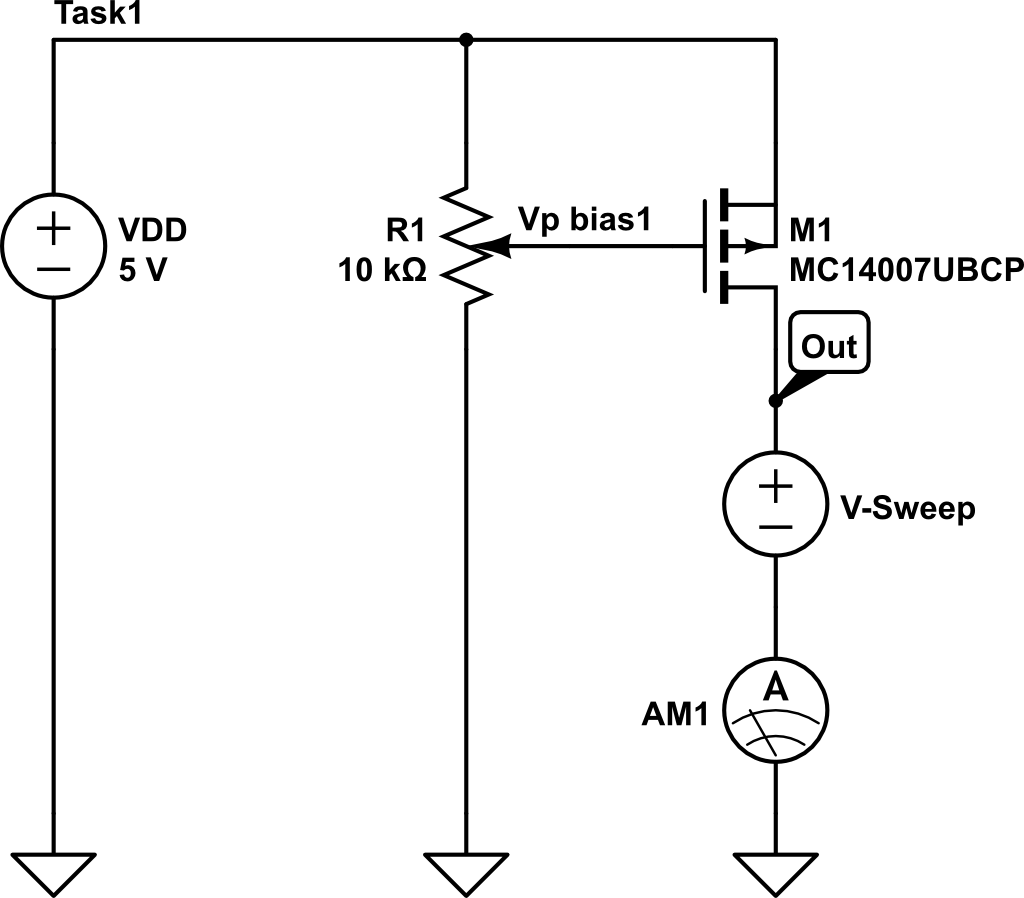
\includegraphics[width=\textwidth]{img/inf4411_lab2_task1_schematics.png}}
  \caption{Transistor setup.}
  \label{fig:sch:task1}	
\end{figure}


\begin{figure}[htbp]
 \centering
  \fbox{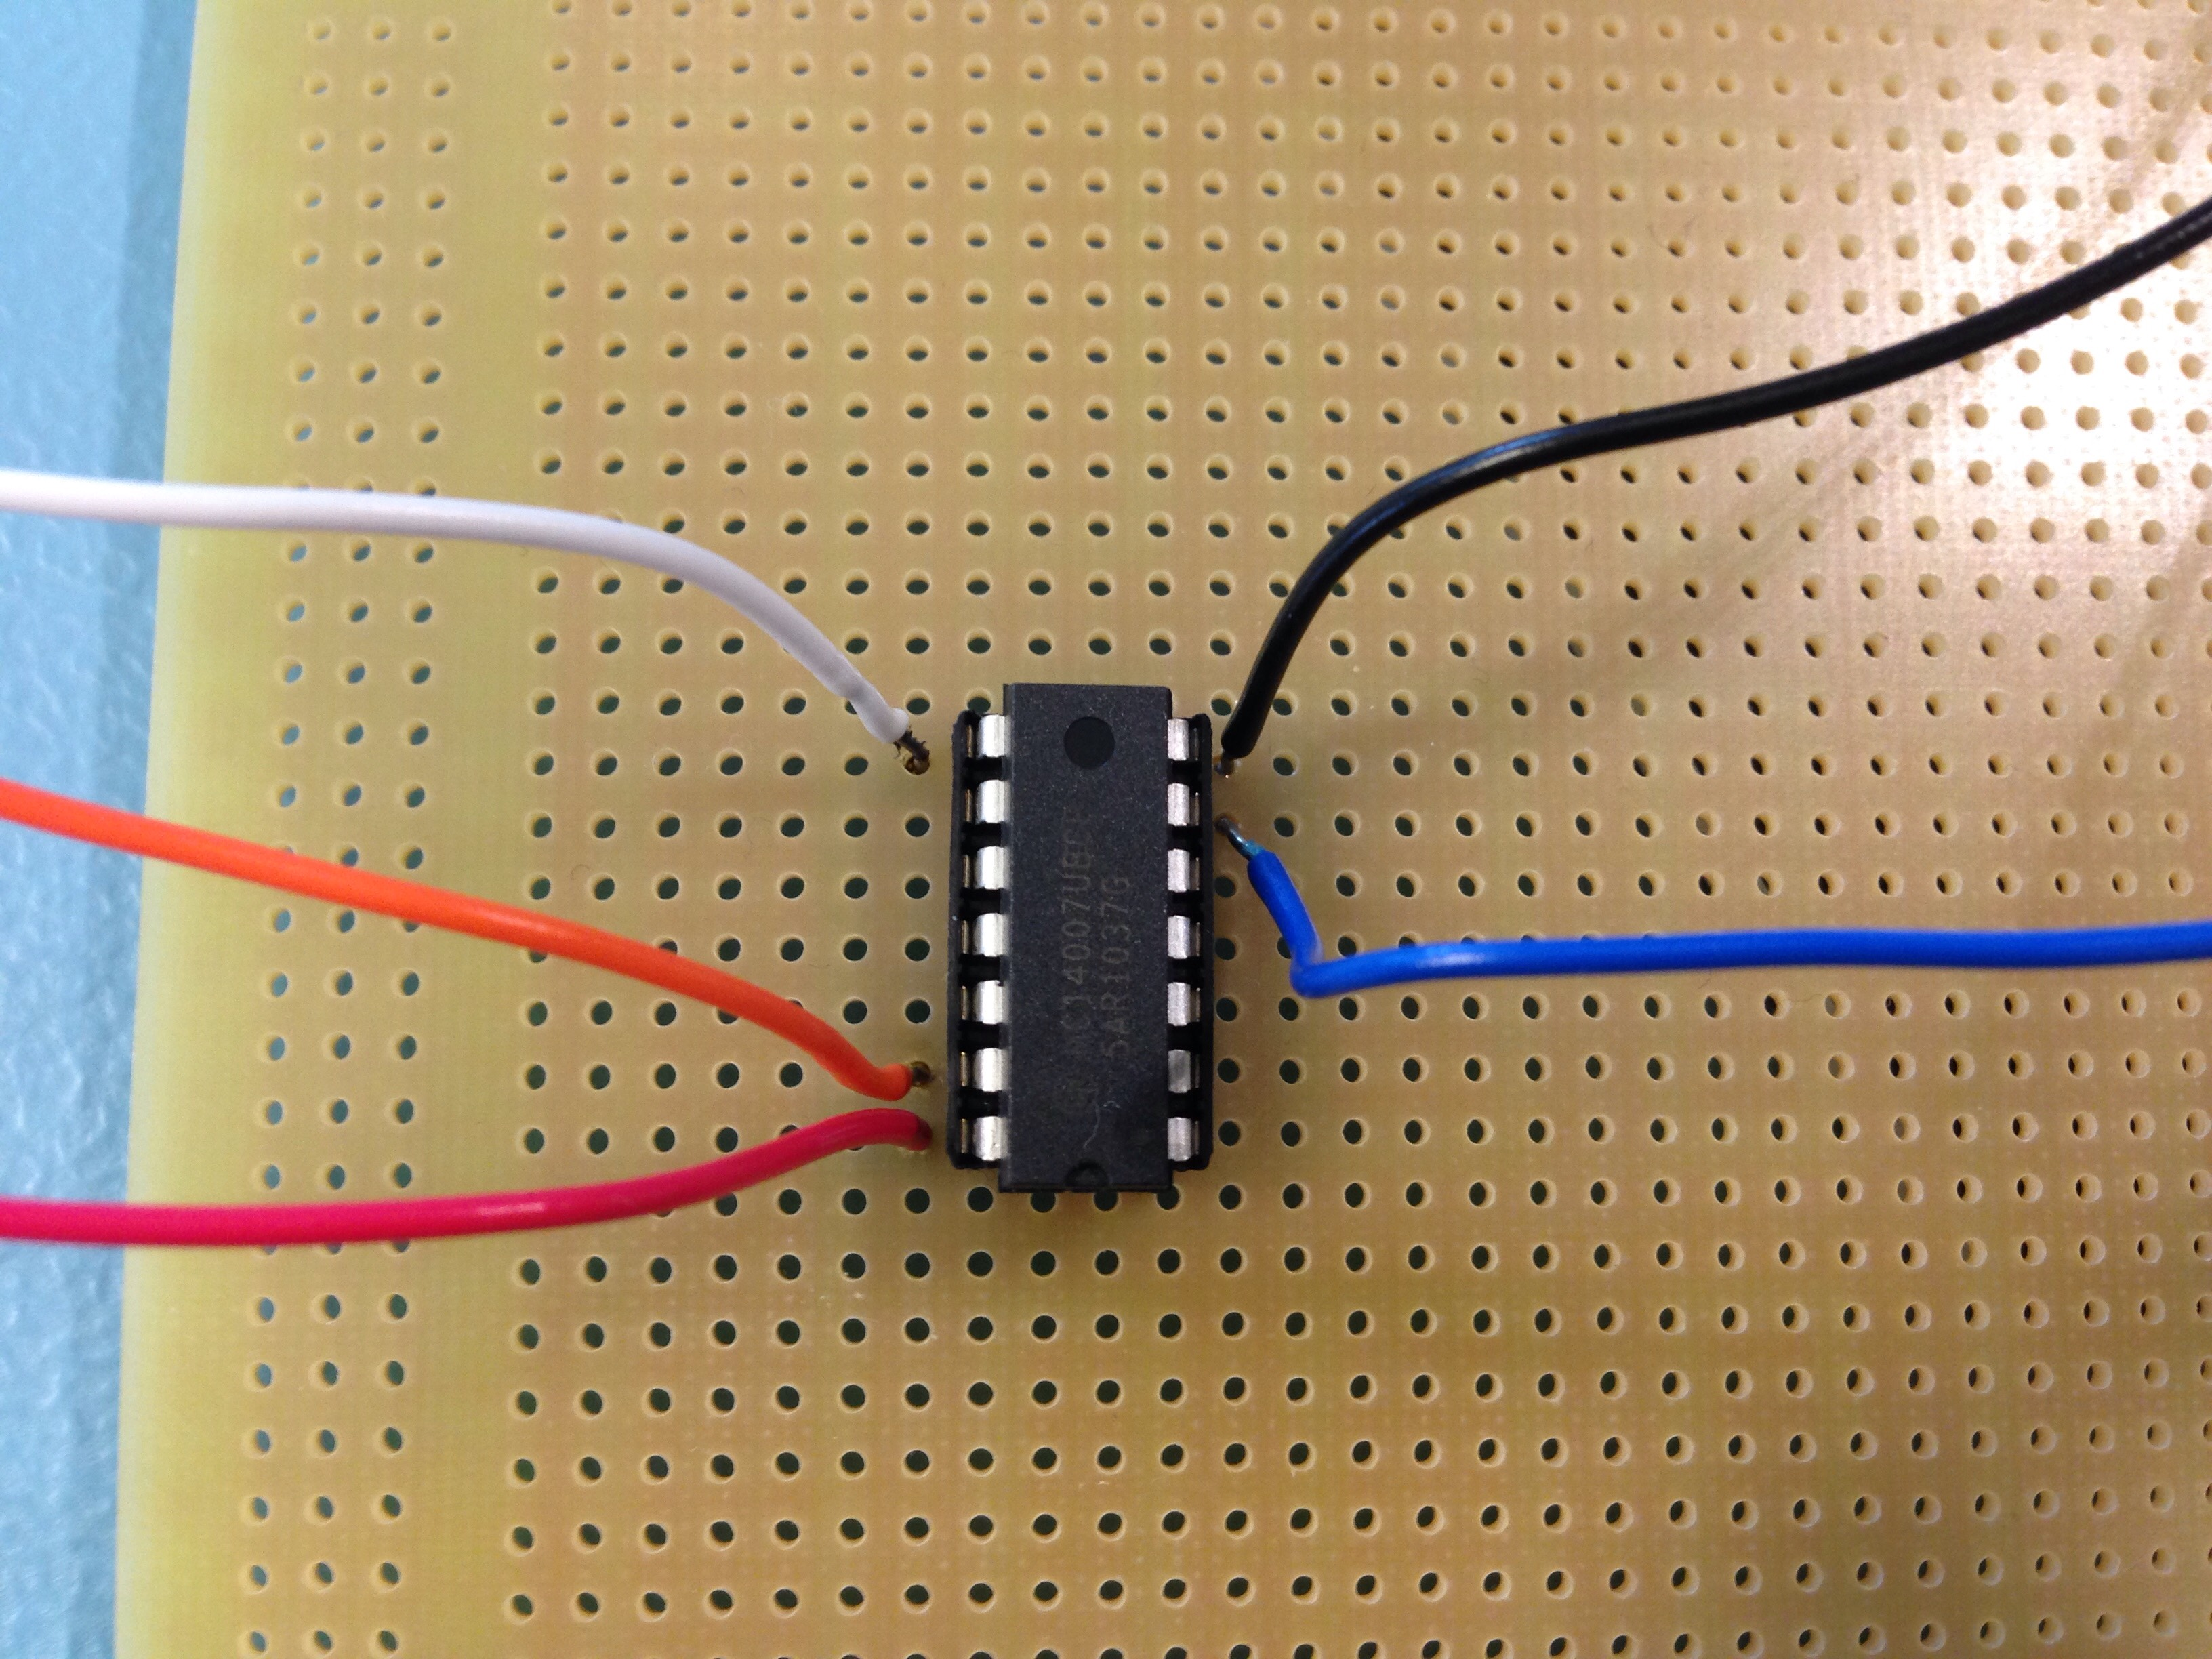
\includegraphics[width=\textwidth]{img/Transistor_setup.jpg}}
  \caption{Transistor setup.}
  \label{fig:tran-setup}	
\end{figure}

\begin{figure}[htbp]
 \centering
  \fbox{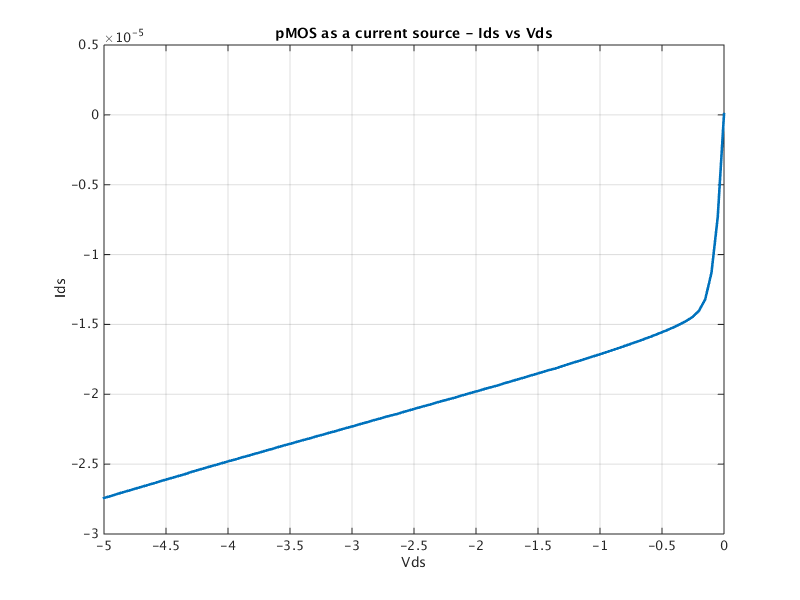
\includegraphics[width=\textwidth]{img/task1_pmos_as_a_current_source.png}}
  \caption{pmos as a current source.}
  \label{fig:pmos-as-current-source}	
\end{figure}

\newpage
\section{Task 2}
Now we extend our circut to a current source with a cascode transistor. This is transistor also need proper biasing. The bias for new transistor is also set by potensiometer as seen i figure *****REF.
Now the minimal voltage difference between Vdd and V$_{p_bias2}$ is ************ in order to get the cuircuit to act as an constant current source.
Figure ***** shows a plot of the \colorbox{blue!30}{output current} as a function of V$_{out}$. \\
The output resistance of this cuircuit is estmated to ***********.\\
The minimial voltage $Vdd - V_{out}$ for the cuircuit is ***************.\\


\colorbox{red!30}{FIXME}\\
Notes:\\
- Used two potentiometers to make the desirable voltage for V$_{p_bias1}$ and V$_{p_bias2}$.\\
- VDD (+25V port) = 5V\\
- V$_{sweep}$ = 2.5V\\
- V$_{p_bias1}$ = 1.196V (From last task)\\
- V$_{p_bias2}$ = 3.39V at 20 $\mu$ A\\
- Minimum voltage different is VDD - V$_{p\_bias2}$ = 5V - 3.39V = \underline{\underline{1.61V}}\\
- Minimun output voltage is 2.83V as seen in Figure \ref{fig:pfet-cascode-pfet}.\\
- Output resistance is 13.35M$\Omega$\\
\\
\colorbox{red!30}{ENDFIXME}\\

Figure \ref{fig:pfet-cascode-pfet} shows plot of output current as function of V$_{out}$.
\begin{figure}[htbp]
 \centering
  \fbox{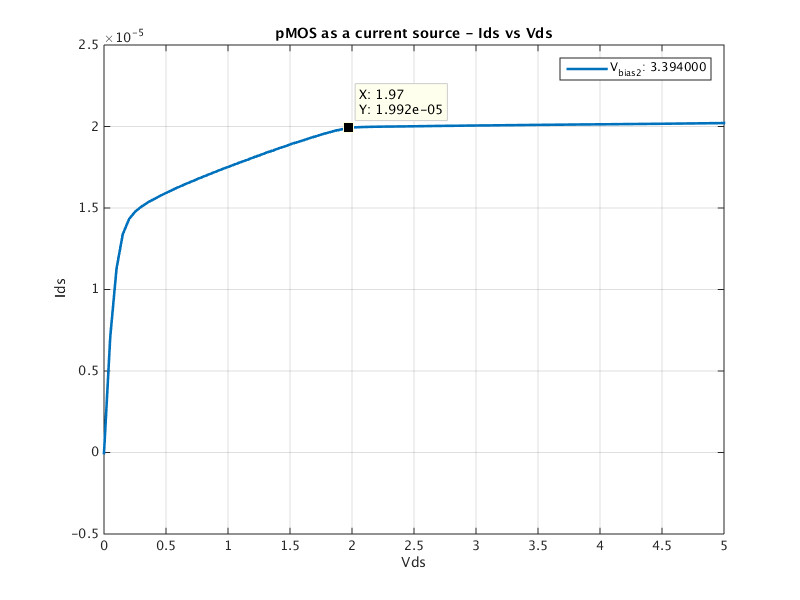
\includegraphics[width=\textwidth]{img/task2_pmos_as_a_current_source.png}}
  \caption{pFET and cascode pFET as a current cource.}
  \label{fig:pfet-cascode-pfet}	
\end{figure}

\section{Task 3}
Using the results form task 1 and task 2 we can estimate values for $V_{eff}$ and the treshold voltage $V_{tp}$.
For task 1 $V_{eff}$ is calculated from the relationship $Vdd - V_{out}$. For task 2 $V_{eff}$ is calculated from the relationship between $V_{out}$ and $V_{p_bias2}$
\\
In task 1 we found the minimal voltage for $Vdd - V_{out}$ to be **************. Using this value to estimate $V_{eff}$ we get ***********.\\
\\
Our results are consistent/not-consistent.....

\newpage
\section{Task 4}
Single stage amplifier.
We now want to determine a good DC voltage for the input for the amplifier. Since our goal is to have an output voltage verry close to $Vdd/2$, we need to find good bias voltages for $V_{n_bias1}$ and $V_{in}$.\\
\\
Doing the same as we did in Task 1 and Task 2, but here we uses nmos transistors instead.\\
\\
1. First we maually find the new V$_n\_bias$ for the first nmos transistor at 20 uA.\\
Uses the same nmos transistor as we did in the lab 1. (port 6(G),7(S) and 8(D))\\
2. Then we use the voltage that we found in the first task and use it in the next task, whis is applying one more nmos transistor. Here we
use the ports 9 (S), 10 (G) and 12 (D). (Reference to picture of setup)


\end{document}
